%!TEX root = ../report.tex
\section{Hardware Overview}
\label{sec:hardware-overview}
The SFM hardware components can be categorized into three main components: sensing part, data storing part, and analytics part. The data flow starts from wired and wireless sensors located across the Netherlands that collect information for monitoring. UAV will also fly to gather additional information if needed. The overview of the hardware and its application interfaces are depicted in \autoref{fig:hardware-archi-schema} below.

% btw is it suppose to be the other way around? sensor monitoring -> analytics-> database ?
%\begin{figure}[H]
%\centering
%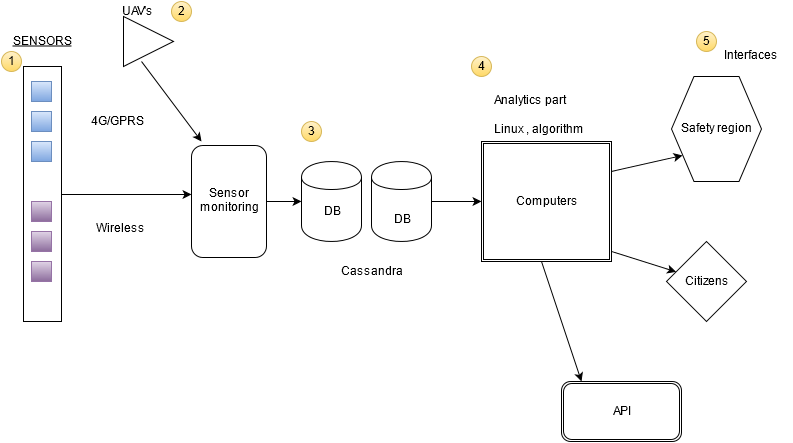
\includegraphics[scale=0.5]{images/HardwareArchitectureOverview.png}
%\caption{Schematic overview of the hardware architecture of \ProjectName{}}
%\label{fig:hardware-archi-schema}
%\end{figure}
\begin{figure}[H]
	\centering
	\includegraphics[scale=0.4]{6-hardware/images/hardwareoverview.png}
	\caption{Schematic overview of the hardware architecture of \ProjectName{}}
	\label{fig:hardware-archi-schema}
\end{figure}

% Need to define where the national and international data centers should be.

The SFM will utilize wired and wireless sensors to monitor water ways and dikes. Wired sensors will be used for dikes monitoring and wireless sensor will be used to monitor water level. Sensors are not directly connected to the main clusters, instead, it will be connected to Arduino and then will be sent periodically using wired Internet connection through telecoms provider's line. An Arduino will be handling several sensors at once.

UAVs will also fly to check reported faulty sensors if needed. UAVs will also be used to take required pictures for further analytics or to examine some portion of the system which is hard or impossible for a personnel to access.

All incoming data will be handled by Data Collecting System in the data centers. This system is also responsible to check any incorrect data input or any faulty sensors. The next part of the hardware is the cluster for carrying out analysis. This will be a collection of servers that are coordinated using clusters. SFM will use another cluster to store important data. This cluster will run Elasticsearch database on top if it.

The last part of the hardware architecture is the third party data gathering cluster. The third party data gathering cluster is responsible for collecting weather forecast and demographic information of the Netherlands. This cluster is also part of the main analytics clusters.

The SFM will have several data centers to keep the system reliable running as reliability and availability is SFM's key drivers. Two of them will be inside the Netherlands and the other one will be located abroad. In this way, the system will be running correctly in case both national data centers go down.